\section{Capa de Enlace: Subcapa de Control de Acceso al Medio (MAC)}

En los canales de difusión generalmente se tiene el problema de que varios usuarios pueden intentar transmitir al mismo tiempo, lo que genera colisiones. Para resolver este problema, se utilizan protocolos de acceso al medio (MAC) que determinan cómo los usuarios comparten el canal. 

La subcapa MAC tiene especial importancia en las LAN, en especial las inalámbricas puesto que el canal inalámbrico es de difusión por naturaleza. Debido a que los canales multiacceso y las LAN están muy relacionados, en esta sección analizaremos las LAN en general.

\subsection{El Problema de Asignación del Canal}

El tema central de esta subcapa es la forma de asignar un solo canal de difusión entre usuarios competidores. El canal podría ser una parte del espectro inalámbrico en una región geográfica, o una fibra óptica en donde se conectan varios nodos. Esto no es importante. En ambos casos, el canal conecta a cada usuario con todos los demás, cualquier usuario que utilice todo el canal interfiere con los demás
que también desean usarlo.

\subsubsection{Asignación Estática del Canal}

La asignación estática consiste en dividir la capacidad total de un único canal de comunicación entre $N$ usuarios competidores, asignando a cada uno una fracción fija y exclusiva del recurso. Esta división se implementa convencionalmente mediante las técnicas de multiplexación que vimos anteriormente, como FDM o TDM. Este esquema resulta eficiente únicamente cuando existe una cantidad pequeña, fija y conocida de usuarios que mantienen una carga de tráfico pesada y constante (por ejemplo, transmisiones de radio FM).

Sin embargo, la asignación estática es ineficiente para las redes de computadoras, donde la naturaleza del tráfico de datos opera en ráfagas de alta intensidad. Bajo este esquema, surgen dos deficiencias críticas:

\begin{itemize}
  \item Si un usuario se encuentra inactivo, su porción de ancho de banda (o ranura de tiempo) se pierde por completo, ya que la división estricta prohíbe que otros emisores la utilicen. En consecuencia, la mayor parte del canal permanece ocioso la mayor parte del tiempo.
  \item Si la cantidad de usuarios que desean transmitir supera el límite físico de particiones $N$, el sistema negará el acceso a los emisores excedentes por falta de espectro asignable, incluso si existen canales de otros usuarios temporalmente inactivos.
\end{itemize}

\subsubsection{Supuestos para la Asignación Dinámica de Canales}

Todo el trabajo hecho en esta área se basa en cinco supuestos clave, que se describen a continuación:

\begin{enumerate}
    \item \textbf{Tráfico independiente:} El modelo consta de $N$ estaciones independientes, cada una generando tramas de forma impredecible pero a una tasa de llegada promedio constante (distribución de Poisson). Tras generar una trama, la estación se bloquea lógicamente y detiene su generación hasta que dicha trama logre transmitirse con éxito.
    \item \textbf{Canal único:} La totalidad de las comunicaciones ocurre sobre un único medio físico compartido. Todas las estaciones transmiten y reciben sobre él.
    \item \textbf{Colisiones observables:} Si dos tramas se transmiten en forma simultánea, se traslapan en el tiempo y la señal resultante se altera. Este evento se llama \textbf{colisión}. Todas las estaciones pueden detectar una colisión que haya ocurrido. Una trama en colisión se debe volver a transmitir después. No hay otros errores, excepto aquéllos generados por las colisiones.
    \item \textbf{Tiempo continuo o ranurado:} Se puede asumir que el tiempo es continuo, en cuyo caso la transmisión de una trama puede comenzar en cualquier momento. Por el contrario, el tiempo se puede ranurar o dividir en intervalos discretos (llamados ranuras). En este caso las transmisiones de las tramas deben empezar al inicio de una ranura. Una ranura puede contener 0, 1 o más tramas, correspondientes a una ranura inactiva, una transmisión exitosa o una colisión, respectivamente. 
    \item \textbf{Detección de portadora o sin detección:} Con el supuesto de detección de portadora, las estaciones pueden saber si el canal está en uso antes de intentar usarlo. Si se detecta que el canal está ocupado, ninguna estación intentará utilizarlo. Si no hay detección de portadora, las estaciones no pueden detectar el canal antes de intentar usarlo. Simplemente transmiten. Sólo después pueden determinar si la transmisión tuvo éxito.
\end{enumerate}

\subsection{Protocolos de Acceso Múltiple}

\subsubsection{ALOHA}

ALOHA fue el primer protocolo MAC diseñado para un medio de difusión compartido (originalmente redes de radio). Analizaremos las dos variantes de este protocolo:

\begin{itemize}
    \item \textbf{ALOHA Puro:} La idea básica es sencilla: cuando una estación tiene una trama para enviar, la transmite inmediatamente al canal. No verifica si el medio está ocupado antes de transmitir. 
    
    Dado que las estaciones transmiten en instantes completamente aleatorios, es inevitable que los tiempos de transmisión de dos o más tramas se superpongan. En ALOHA puro, si esto ocurre, decimos que las tramas colisionan y se corrompen mutuamente. La estación central al recibir una trama transmite a todas las estaciones la misma, por lo tanto, si una estación no recibe la trama que envió, sabe que ocurrió una colisión y que su trama se perdió.
    
    Si la trama fue destruida, el emisor simplemente espera un tiempo aleatorio y la envía de nuevo. El tiempo de espera debe ser aleatorio o las mismas tramas chocarán una y otra vez, en sincronía. Los sistemas en los cuales varios usuarios comparten un canal común de modo tal que puede dar pie a conflictos se conocen como sistemas de \textbf{contención}.

    Lo malo de esto es que no importa que tanto se solapen las tramas, con que al menos un bit se superponga, la trama se pierde.
    
    \item \textbf{ALOHA Ranurado:} Para mejorar el ineficiente rendimiento del ALOHA puro, se introdujo una restricción temporal. En ALOHA ranurado, el tiempo continuo se divide en intervalos discretos (ranuras) de tamaño igual al tiempo de transmisión de una trama estándar.
    
    La nueva regla de operación exige que las estaciones estén sincronizadas: cuando una estación genera una trama, no puede transmitirla inmediatamente. Debe esperar obligatoriamente al inicio de la siguiente ranura de tiempo. Para lograr esto, se utiliza una estación especial que transmite una señal al comienzo de cada intervalo.
    
    Esta discreción temporal altera drásticamente la probabilidad de colisiones. Al obligar a que todas las transmisiones comiencen exactamente en el mismo instante, se elimina la posibilidad de solapamientos parciales. Las tramas o colisionan por completo (si dos o más estaciones transmiten en la misma ranura), o no colisionan en absoluto. Al reducir el periodo de vulnerabilidad exactamente a la mitad en comparación con el modelo puro, ALOHA ranurado duplica la eficiencia máxima teórica.
\end{itemize}


\subsubsection{Protocolos de Acceso Múltiple con Detección de Portadora}

La ineficiencia de los sistemas ALOHA radica en que las estaciones no conocen el estado del canal. En muchas redes (particularmente las redes LAN alámbricas), es posible que las estaciones escuchen el canal antes de actuar, mecanismo que se denomina \textbf{detección de portadora}. Los protocolos que utilizan esta característica adaptan su comportamiento para evitar colisiones obvias, mejorando el rendimiento del canal. 

La familia de protocolos \textbf{CSMA} (Carrier Sense Multiple Access) implementan esta idea mediante sus distintas variantes:

\begin{itemize}
    \item \textbf{CSMA persistente-1:} Cuando una estación tiene datos por enviar, escucha el canal. Si está inactivo, transmite inmediatamente. Si está ocupado, la estación se queda escuchando continuamente hasta que el canal se libere, en ese preciso instante, transmite su trama (con probabilidad de 1, de ahí el nombre). Esto evita colisiones con una transmisión en curso, pero si dos o más estaciones están esperando a que termine una transmisión, ambas intentarán transmitir exactamente al mismo tiempo cuando el canal se libere.

    \item \textbf{CSMA no persistente:} Busca solucionar el problema del CSMA persistente-1 siendo menos egoísta. Si una estación desea transmitir y encuentra el canal ocupado, en lugar de quedarse esperando a que finalice la transmisión actual, espera un periodo de tiempo aleatorio y recién entonces vuelve a escuchar el canal. Esto reduce las colisiones, pero introduce retraso.

    \item \textbf{CSMA persistente-p:} Diseñado para canales de tiempo ranurado. Si la estación encuentra el canal inactivo, transmite con una probabilidad $p$. Si no lo hace (con probabilidad $q = 1-p$), espera a la siguiente ranura temporal. Si en esa ranura el canal sigue libre, vuelve a aplicar la lógica anterior. Si el canal está ocupado, espera un tiempo aleatorio e inicia el proceso nuevamente. Es la base conceptual de las redes Wi-Fi (IEEE 802.11).
\end{itemize}

\textbf{CSMA con detección de colisiones}

CSMA evita colisiones al inicio, pero si dos estaciones detectan el canal libre y transmiten simultáneamente, sus señales de todas formas chocarán. En los esquemas anteriores, las estaciones terminan de transmitir toda su trama a pesar de que ya está corrupta, desperdiciando ancho de banda. 

CSMA/CD mejora este comportamiento añadiendo \textbf{detección de colisiones}. Mientras una estación está transmitiendo, el hardware escucha analógicamente la línea. Si la señal que lee es distinta a la que está enviando, sabe inmediatamente que ha ocurrido una colisión. En ese instante, la estación deja de transmitir.

Un aspecto vital en CSMA/CD es que la detección de una colisión no es instantánea debido al retardo de propagación de la señal. Si el tiempo que tarda una señal en viajar de un extremo al otro de la red es $\tau$, en el peor de los casos una estación que inició una transmisión tardará hasta $2\tau$ (el tiempo de viaje de ida y vuelta) en enterarse de que colisionó. Por lo tanto, una estación solo puede estar segura de que tomó el canal (y que nadie más transmitirá) tras haber transmitido durante un tiempo $2\tau$ sin detectar conflictos.

Este protocolo es la base de la clásica LAN Ethernet.

\subsubsection{Protocolos Libres de Colisiones}

Aunque CSMA/CD mejora drásticamente el rendimiento frente al modelo ALOHA, las colisiones siguen ocurriendo durante el periodo de contención, lo cual degrada el desempeño cuando la red tiene una carga alta. Los protocolos libres de colisiones resuelven la contención de manera que el solapamiento de tramas sea imposible por diseño.

\begin{itemize}
    \item \textbf{Protocolo de mapa de bits:} El periodo de contención se divide en $N$ ranuras de tiempo estandarizadas, una para cada estación. Si la estación $j$ desea transmitir, emite un bit de valor 1 durante su ranura respectiva. Al finalizar el periodo de las $N$ ranuras, todas las estaciones saben de forma determinista quién desea transmitir. Las estaciones interesadas transmiten sus tramas en estricto orden numérico secuencial. Evita colisiones absolutas a costa de la sobrecarga obligatoria de transmitir el mapa de bits completo antes de cada ronda de datos.
    
    En la siguiente figura se muestra un ejemplo de mapa de bits con 8 estaciones.
    \begin{figure}[h]
        \centering
        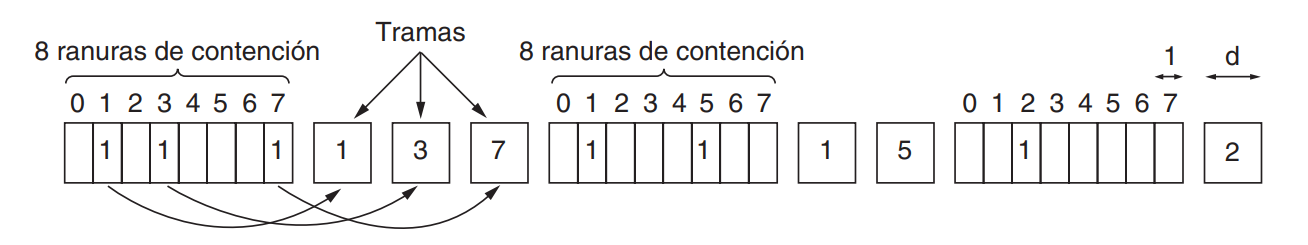
\includegraphics[width=0.8\textwidth]{imgs/4.2.png}
    \end{figure}
    \item \textbf{Paso de token:} Utiliza un mensaje de control lógico especial denominado token. Las estaciones se organizan (física o lógicamente) en una topología de anillo. El token circula sistemáticamente de una estación a otra. Únicamente la estación en posesión del token está autorizada a transmitir datos sobre el canal. Al finalizar, pasa el token.
    \item \textbf{Conteo descendente binario:} Cada estación posee una dirección binaria única de longitud fija. Las estaciones que desean transmitir difunden su dirección bit por bit sincronizadamente, empezando por el bit más significativo. Las direcciones se combinan en el canal mediante una función OR booleana. Si una estación transmite un 0 pero lee un 1 del canal, comprende que compite contra una estación con una dirección mayor, en ese instante se rinde y abandona la contención. La estación con la dirección numérica más alta siempre gana el acceso al medio sin colisionar datos. Este protocolo asume de manera implícita que los retardos de transmisión son insignificantes, de manera que todas las estaciones ven los bits instantáneamente.
\end{itemize}

\subsubsection{Protocolos de Contención Limitada}

Los protocolos de contención pura (como CSMA) ofrecen un buen rendimiento frente a cargas ligeras, pero son deficientes bajo carga alta por el aumento de colisiones. Inversamente, los protocolos libres de colisiones garantizan eficiencia bajo carga saturada, pero generan retrasos innecesarios a carga baja.

Los protocolos de contención limitada buscan combinar las ventajas de ambos, decidiendo dinámicamente qué estaciones pueden competir por el canal según la carga de tráfico.

El \textbf{protocolo de recorrido de árbol adaptable} modela a las estaciones como las hojas de un árbol binario. En la primera ranura posterior a una transmisión exitosa, todas las estaciones (el nodo raíz) intentan transmitir. Si ocurre una colisión, en la siguiente ranura solo las estaciones en la mitad izquierda del árbol (las estaciones bajo ese subárbol) podrán competir. Si vuelve a colisionar, se restringe a la mitad izquierda de esa mitad. Cuando un grupo logra transmitir con éxito o dejar el canal inactivo, el algoritmo cede el turno a la mitad derecha del nivel correspondiente. Este mecanismo ajusta la carga de la contención dinámicamente según el nivel de tráfico.


\subsubsection{Protocolos de LAN Inalámbrica}

Los protocolos CSMA tradicionales fueron diseñados para redes alámbricas, asumiendo que todas las estaciones pueden escucharse entre sí. En los entornos inalámbricos de radio, la potencia de la señal decae rápidamente con la distancia. Esta limitación física invalida los supuestos alámbricos e introduce dos anomalías estructurales que degradan el rendimiento:

\begin{itemize}
    \item \textbf{El problema de la terminal oculta:} Supongamos que la estación $A$ está transmitiendo hacia $B$. Una estación $C$, también desea transmitir a $B$. La estación $C$ escucha el canal antes de transmitir, pero dado que $A$ está fuera de su rango de radio, $C$ no detecta portadora. $C$ concluye erróneamente que el medio está inactivo e inicia su transmisión hacia $B$. Ambas señales colisionan en el receptor $B$, destruyendo la información.

    \item \textbf{El problema de la terminal expuesta:} Supongamos que $B$ está transmitiendo hacia $A$. La estación $C$, que es vecina de $B$, desea iniciar una transmisión hacia una estación lejana $D$. $C$ escucha el canal, detecta la transmisión en curso de $B$, asume que el medio está ocupado y pospone su envío. Sin embargo, este aplazamiento es innecesario y desperdicia ancho de banda: la transmisión de $C$ hacia $D$ no interferiría en absoluto con la recepción que $A$ está haciendo de $B$, porque $A$ está fuera del rango de $C$.
\end{itemize}

Para resolver estas deficiencias, surge el protocolo \textbf{MACA (Multiple Access with Collision Avoidance)}. El concepto en que se basa es que el emisor estimule al receptor para que envíe una trama corta, de manera que las estaciones cercanas puedan detectar esta transmisión y
eviten ellas mismas hacerlo durante la siguiente trama de dato (grande). Se utiliza esta técnica en vez de la detección de portadora.

El proceso de transmisión de datos mediante MACA consiste en:

\begin{enumerate}
    \item Antes de enviar datos, el emisor transmite una trama de control muy corta denominada \textbf{RTS} (Request To Send), indicando explícitamente la longitud de la trama de datos que desea enviar.
    \item Si el receptor está inactivo y recibe el RTS, responde emitiendo una trama \textbf{CTS} (Clear To Send), copiando en ella la longitud anunciada de los datos.
    \item Al recibir el CTS, el emisor inicia inmediatamente la transmisión de los datos reales.
\end{enumerate}

Este mecanismo de intercambio protege el canal controlando a las estaciones vecinas de la siguiente manera:
\begin{itemize}
    \item Resolución de la terminal oculta: Cualquier estación (como $C$ en el primer ejemplo) que escuche el CTS sabe que una estación cercana está a punto de recibir datos. Por lo tanto, extrae la longitud de los datos de la trama CTS y permanece obligatoriamente en silencio durante ese lapso de tiempo.
    \item Resolución de la terminal expuesta: Si una estación escucha un RTS pero no escucha un CTS (como $C$ en el segundo ejemplo), deduce algebraicamente que está cerca del emisor pero lejos del receptor objetivo. En consecuencia, sabe que puede transmitir libremente sin causar colisiones en el destino de esa transmisión, optimizando la concurrencia espacial de la red.
\end{itemize}

Cabe destacar que las propias tramas RTS aún pueden colisionar (si dos estaciones inician el protocolo hacia el mismo destino simultáneamente). Ante esta colisión, el emisor no recibirá el CTS esperado, por lo que abortará el intento, aplicará un tiempo de espera aleatorio y reintentará más tarde.

\subsection{Ethernet}

Ethernet es el estándar dominante en redes de área local (LAN) alámbricas. Existen dos tipos de Ethernet: Ethernet clásica, que resuelve el problema de acceso múltiple mediante el uso de las técnicas que hemos estudiado en esta sección; el segundo tipo es la Ethernet conmutada, en donde los dispositivos llamados switches se utilizan para conectar distintas computadoras. Es importante mencionar que, aunque se hace referencia a ambas como Ethernet, son muy diferentes. La Ethernet clásica es la forma original que operaba a tasas de transmisión de 3 a 10 Mbps. La Ethernet conmutada es en lo que se convirtió la Ethernet y opera a 100, 1000 y 10000 Mbps. Actualmente, en la práctica sólo se utiliza Ethernet conmutada.

A nivel físico, la Ethernet clásica utiliza un cable coaxial grueso o delgado, mientras que la Ethernet conmutada utiliza cables de par trenzado o fibra óptica. Se tendía un cable a lo largo de un edificio y se conectaban las computadoras a este cable mediante un conector. La Ethernet conmutada utiliza un dispositivo mediador llamado switch, que tiene varios puertos, cada uno de los cuales se conecta a una computadora mediante un cable de par trenzado o fibra óptica.


\subsubsection{Formato de la Trama y Restricciones Físicas}

La subcapa MAC de Ethernet encapsula los paquetes de la capa de red en tramas con la siguiente estructura básica:

\begin{itemize}
    \item \textbf{Preámbulo:} Secuencia de 8 bytes (alternando unos y ceros, finalizando en 11) utilizada para la sincronización de reloj en el hardware receptor.
    \item \textbf{Direcciones MAC:} Dos campos de 6 bytes que identifican unívocamente la dirección física de destino y de origen.
    \item \textbf{Tipo/Longitud (2 bytes):} Indica el protocolo de capa de red encapsulado (ej. IPv4, ARP) o, en implementaciones antiguas, la longitud de la carga útil.
    \item \textbf{Datos:} Carga útil proveniente de la capa superior. Está acotada a un máximo estricto de 1500 bytes.
    \item \textbf{Relleno:} Bytes inactivos añadidos si la carga útil es insuficiente para que la trama alcance el tamaño mínimo requerido.
    \item \textbf{Suma de verificación (4 bytes):} Un código CRC-32 (Cyclic Redundancy Check) evaluado por el hardware receptor para detectar corrupciones de bits.
\end{itemize}

\textbf{Límite mínimo de trama:} Para que el mecanismo CSMA/CD detecte colisiones algorítmicamente, la transmisión debe durar al menos el tiempo de propagación de ida y vuelta de la red ($2\tau$). Esto garantiza que el emisor siga transmitiendo (y pueda sensar la colisión en el nivel de voltaje) cuando la perturbación regrese a él. En la Ethernet clásica a 10 Mbps, este requerimiento impone un tamaño mínimo de trama de \textbf{64 bytes}. Toda trama inferior recibida se descarta.

\subsubsection{Algoritmo de Retroceso Exponencial Binario}

Para gestionar la contención del canal, la Ethernet clásica implementa CSMA/CD persistente-1 regido por el algoritmo de retroceso exponencial binario. Este algoritmo, se escogió para adaptar en forma dinámica el número de estaciones que intentan transmitir.

El algoritmo funciona de la siguiente manera:

Tras detectar una colisión, el tiempo se divide en ranuras discretas (equivalentes al tiempo de transmisión de 512 bits, es decir, el tamaño mínimo de trama). Ante la $i$-ésima colisión consecutiva de una misma trama, la estación elige uniformemente un número aleatorio de ranuras de espera en el intervalo $[0, 2^i - 1]$. 

El límite superior del intervalo crece exponencialmente para dispersar los intentos de transmisión y evitar que las estaciones colisionen repetidamente bajo alta carga. El exponente máximo se encuentra tras la décima colisión (congelando el intervalo en $[0, 1023]$). Si el proceso fracasa tras 16 colisiones consecutivas, el hardware aborta la transmisión y notifica la falla a la capa superior.

\subsubsection{Evolución Tecnológica}

El diseño de Ethernet escaló en ancho de banda manteniendo invariable el formato de trama para garantizar la compatibilidad hacia atrás.

\begin{itemize}
    \item \textbf{Ethernet Conmutada:} Se sustituyen los concentradores (hubs) por conmutadores (switches). Un switch aísla eléctricamente cada puerto, fragmentando el dominio de colisión global. Un switch se encarga de tomar un paquete recibido por un puerto y redireccionarlo al destino correspondiente. Al interconectar dispositivos punto a punto contra el switch, la red opera en modo \textbf{Full-Duplex} (transmisión y recepción simultáneas en canales físicos separados). Físicamente, las colisiones se vuelven imposibles y el algoritmo CSMA/CD se deshabilita.
    
    \item \textbf{Fast Ethernet (100 Mbps):} Multiplicó la tasa de transferencia por un factor de 10. Para preservar el límite de CSMA/CD y mantener el tamaño mínimo de 64 bytes operando en Half-Duplex, el diámetro físico máximo permitido para la red se redujo en un factor de 10.
    
    \item \textbf{Gigabit Ethernet (1 Gbps) y superiores:} Introdujo mecanismos lógicos (extensión de portadora y ráfagas de tramas) para evitar que el diámetro máximo de red colapsara a unos impracticables 25 metros (esto debido a la necesidad de reducir el diámetro físico con el objetivo de aumentar la velocidad de transmisión). Sin embargo, en implementaciones reales, Gigabit y 10-Gigabit Ethernet se despliegan exclusivamente sobre hardware conmutado en modo Full-Duplex, volviendo obsoleto el uso de CSMA/CD.
\end{itemize}

\begin{obs}
  Antes que los switches, se utilizaban \textbf{concentradores (hubs)} para interconectar las computadoras. Un concentrador es un dispositivo que repite la señal que recibe en todos sus puertos, por lo que todas las computadoras conectadas a él comparten el mismo canal de comunicación. Esto genera colisiones y obliga a utilizar CSMA/CD.
\end{obs}

\subsection{Redes LAN Inalámbricas}

El estándar IEEE 802.11 (Wi-Fi), define las especificaciones para las redes de área local inalámbricas. A diferencia de las redes cableadas, el medio inalámbrico presenta altas tasas de error, interferencias, y las problemáticas estructurales de las terminales ocultas y expuestas, requiriendo un diseño  sustancialmente distinto.

\subsubsection{Arquitectura del 802.11}

El estándar define dos modos operativos fundamentales:
\begin{itemize}
    \item \textbf{Modo de Infraestructura:} Las máquinas se comunican de manera inálambrica a través de un AP (Access Point). El AP actúa como puente entre la red inalámbrica y una red cableada subyacente, denominada DS (Distribution System). El conjunto formado por un AP y sus estaciones asociadas se denomina BSS (Basic Service Set).
    \item \textbf{Modo Ad-hoc:} Las estaciones se comunican directamente entre sí sin la intervención de una infraestructura central o AP. Este modelo conforma un IBSS (Independent Basic Service Set). No es muy popular debido a que no permite la conexión a Internet ni a otras redes cableadas (solo sirve para comunicaciones locales).
\end{itemize}

Todas las técnicas 802.11 usan radios de corto alcance para transmitir en frecuencias de 2.4 GHz o 5 GHz, con un alcance típico de 30 a 100 metros. La ventaja de estas frecuencias es que no requieren licencia, pero la desventaja es que son muy susceptibles a interferencias de otros dispositivos.

\subsubsection{El Protocolo de la Subcapa MAC}

El protocolo de la subcapa MAC para el estándar 802.11 es muy diferente al de Ethernet, debido a la naturaleza half-dúplex de los dispositivos de comunicación inalambrica, lo cual significa que no pueden transmitir y escuchar ráfagas de ruido al mismo tiempo en una sola frecuencia. Por lo tanto, se implementa \textbf{CSMA/CA} (Carrier Sense Multiple Access with Collision Avoidance). Este protocolo es similar al CSMA/CD de Ethernet, con detección del canal antes de enviar y retroceso exponencial después de las colisiones. Sin embargo, una estación que desee enviar una trama empieza con un retroceso aleatorio (excepto en el caso en que no haya utilizado el canal recientemente y éste se encuentre inactivo). La estación espera hasta que el canal está inactivo, para lo cual detecta que no hay señal durante un periodo corto y realiza un conteo descendente de las ranuras inactivas, haciendo pausa cuando se envían tramas. Envía su trama cuando el contador llega a 0. Si la trama logra pasar, el destino envía de inmediato una \textbf{confirmación de recepción} corta. La falta de una confirmación de recepción se interpreta como si hubiera ocurrido un error, sea una colisión o cualquier otra cosa. En este caso, el emisor duplica el periodo de retroceso e intenta de nuevo, continuando con el retroceso exponencial como en Ethernet, hasta que la trama se transmita con éxito o se llegue al número máximo de retransmisiones.

El estándar soporta dos mecanismos de control de acceso al medio que pueden coexistir:
\begin{itemize}
    \item \textbf{DCF (Distributed Coordination Function):} Es el modo de contención predeterminado, basado en CSMA/CA. Emplea detección de portadora tanto física como virtual.
    \item \textbf{PCF (Point Coordination Function):} Es un modo opcional libre de colisiones. El AP actúa como coordinador central realizando un sondeo  secuencial a las estaciones para otorgarles acceso exclusivo al canal, acotando los retardos para aplicaciones en tiempo real.
\end{itemize}

\textbf{Detección de Portadora Virtual (NAV)}\\
Para reducir las ambigüedades con respecto a qué estación va a transmitir, el 802.11 define la detección del canal como un proceso que consiste tanto de una detección física como de una detección virtual. En la detección física sólo se verifica el medio para ver si hay una señal válida. Para la detección virtual, el estándar establece que toda trama transmitida debe incluir un campo de duración. Cada estación mantiene una variable local denominada \textbf{NAV} (Network Allocation Vector), que registra el tiempo que el canal permanecerá ocupado. Si una estación escucha cualquier trama que no sea para ella, actualiza su NAV y suspende toda transmisión analógica hasta que este temporizador llegue a cero. Hay un mecanismo RTS/CTS opcional que usa el NAV para evitar que las terminales envíen tramas al mismo tiempo como terminales ocultas.

\textbf{InterFrame Spacing (IFS)}\\
Para establecer prioridades deterministas en el acceso al canal, 802.11 exige que las estaciones esperen intervalos de tiempo específicos (con el canal inactivo) antes de poder transmitir:
\begin{itemize}
    \item \textbf{SIFS (Short IFS):} El intervalo más corto. Reservado para tramas de máxima prioridad (ACKs, CTSs o fragmentos subsiguientes de una ráfaga de datos), garantizando que ninguna otra estación intercepte el canal durante una transacción.
    \item \textbf{DIFS (DCF IFS):} Intervalo estándar. Utilizado por las estaciones operando en modo DCF para intentar transmitir tramas de datos nuevas.
    \item \textbf{EIFS (Extended IFS):} El intervalo más largo. Obligatorio para una estación que acaba de recibir una trama corrupta, otorgando tiempo a la red para completar la secuencia de error sin interferencias.
\end{itemize}

\subsubsection{Estructura de la Trama 802.11}

El estándar define tres clases principales de tramas en el medio inalámbrico: \textbf{de datos}, \textbf{de control} y \textbf{de administración}.

El formato general de una trama de datos consta de los siguientes campos fundamentales:

\begin{itemize}
    \item \textbf{Control de Trama (2 bytes):} Contiene subcampos críticos para la lógica del protocolo, tales como la versión del protocolo, el tipo de trama (de control, de datos o de administración), el subtipo (por ej, RTS o CTS), entre otros.
    \item \textbf{Duración (2 bytes):} Especifica el tiempo exacto (en microsegundos) que la trama de datos y su respectivo acuse de recibo  ocuparán en el canal. Este valor es leído por todas las estaciones circundantes para configurar su temporizador NAV.
    \item \textbf{Direcciones (Hasta 4 campos de 6 bytes):} A diferencia de Ethernet (que emplea estrictamente dos direcciones), el ruteo a través de AP en 802.11 requiere aislar lógicamente los saltos. Los campos especifican: Dirección de destino final, Dirección de origen inicial, Dirección del receptor inmediato (el AP) y Dirección del transmisor inmediato.
    \item \textbf{Secuencia (2 bytes):} Numera las tramas de manera que se puedan detectar tramas duplicadas. De los 16 bits disponibles, 4 identifican el fragmento y 12 transportan un número que avanza con cada nueva transmisión.
    \item \textbf{Datos (0 a 2312 bytes):} Contiene la carga útil. Los primeros bytes de este campo emplean el formato LLC para identificar unívocamente al protocolo de capa superior (por ejemplo, IPv4) al que deben entregarse los datos.
    \item \textbf{Secuencia de Verificación (4 bytes):} Emplea un código CRC para el control de errores, garantizando la integridad de los bits recibidos.
\end{itemize}

Las tramas de administración tienen el mismo formato que las tramas de datos, además de un formato para la parte de los datos que varía con el subtipo. 

Las tramas de control son cortas. Al igual que todas las tramas, tienen los campos Control de trama, Duración y Secuencia de verificación de trama. Sin embargo, ellas pueden tener sólo una dirección y ninguna porción de datos. La mayoría de la información clave se transmite mediante el campo Subtipo
(por ejemplo, ACK, RTS y CTS).

\subsubsection{Servicios del Estándar 802.11}

El estándar exige que los clientes, los puntos de acceso y la red que los conecta implementen un conjunto de servicios para operar funcionalmente como una LAN inalámbrica. Estos servicios se dividen de la siguiente manera:

\begin{itemize}
    \item \textbf{Gestión de Conexión y Movilidad:}
    \begin{itemize}
        \item Asociación: Procedimiento inicial mediante el cual una estación negocia sus capacidades (tasas de transmisión, arreglos de seguridad) y se vincula a un AP para acceder a la red.
        \item Reasociación: Permite a una estación transferir su conexión de un AP a otro dentro de la misma red inalámbrica.
        \item Desasociación: Ruptura del vínculo entre la estación y el AP.
    \end{itemize}

    \item \textbf{Seguridad:}
    \begin{itemize}
        \item Autenticación: Validación de las credenciales de la estación. Si la red está abierta, cualquiera puede utilizarla. En caso contrario, se requiere autenticación para acceder a la red. El esquema actual recomendado es \textbf{WPA2} (estándar 802.11i), que reemplazó al algoritmo WEP (Wired Equivalent Privacy). En el WPA2, el AP se puede comunicar con un servidor de autentificación que tenga una base de datos con nombres de usuario y contraseñas para determinar si la estación puede acceder a la red. Como alternativa se puede configurar una contraseña de red. Se intercambian varias tramas entre la estación y el AP donde la estación debe demostrar que tiene las credenciales apropiadas. Este intercambio ocurre después de la asociación.
        \item Privacidad: Dado que el espectro de radio es inherentemente público, este servicio cifra las cargas útiles de las tramas (usualmente mediante el estándar AES (Advanced Encryption Standard) bajo WPA2) para asegurar la confidencialidad.
    \end{itemize}

    \item \textbf{Enrutamiento y Entrega de Datos:}
    \begin{itemize}
        \item Servicio de Distribución: Determina cómo encaminarlas. Si el destino es local para el AP, las tramas se pueden enviar en forma directa por el aire. En caso contrario, habrá que reenviarlas por la red alámbrica.
        \item Servicio de Integración: Realiza las traducciones de formato de trama y direccionamiento necesarias para inyectar los paquetes en redes con arquitecturas distintas (por ejemplo, hacia Internet vía Ethernet).
        \item Entrega de Datos: Transmisión y recepción de las cargas útiles.
    \end{itemize}
\end{itemize}

\subsection{Bluetooth (CREO QUE NO ENTRA, NO C DSP VEO)}
